% =====================================================================
% TEMPLATE SWITCH: leave \naturetrue commented for LoG; uncomment it for
% Springer Nature / Nature Portfolio (sn-jnl class, sn-nature reference style).
% Everything below branches on \ifnature; nothing else needs editing.
% =====================================================================
\newif\ifnature
\newif\ifnatureprint
% \naturetrue
% \natureprinttrue	% with \naturetrue: preview at Nature's printed page width
						% (two 89 mm columns, 183 mm text block; figures span both columns)

% Both classes load xcolor; pass extra options here, before the class, to avoid an option clash.
\PassOptionsToPackage{table}{xcolor}        % \rowcolors / \rowcolor in tables

\ifnature
  % --- Springer Nature (template v3.1, Dec 2024) ---------------------------
  % sn-jnl already loads hyperref, geometry and natbib[numbers,sort&compress],
  % and sets \bibliographystyle{sn-nature}. Do NOT load natbib or hyperref yourself.
  % The submission template is a generic single column with a 31 pc (131 mm) text width,
  % not Nature's printed layout, so figures drawn at 183 mm are shown at ~72% size.
  \ifnatureprint
    \documentclass[pdflatex,sn-nature,iicol]{sn-jnl}
    \geometry{text={183mm,247mm},columnsep=5mm,bindingoffset=0mm,hcentering}
    \setlength\columnhsize{89mm}
  \else
    \documentclass[pdflatex,sn-nature]{sn-jnl}
    % \documentclass[pdflatex,sn-nature,lineno]{sn-jnl}	% with line numbers
    % \documentclass[pdflatex,sn-nature,referee]{sn-jnl}	% double-spaced referee copy
  \fi
  \usepackage{xcolor}
  \usepackage{amsmath}
\else
  % --- LoG 2025 --------------------------------------------------------------
  \documentclass{article}
  \usepackage{log_2025}						% for camera-ready version
  % \usepackage[review]{log_2025}			% for anonymous submission to proceedings track
  % \usepackage[review,eabstract]{log_2025}	% for anonymous submission to extended abstract track
  % \usepackage[preprint]{log_2025}			% for preprint version
  % \usepackage[eabstract]{log_2025}		% for accepted extended abstract papers
  % Citation colour: the style file sets citecolor=NavyBlue (near-black); override it here
  % (any xcolor svgnames colour, e.g. RoyalBlue, MediumBlue, Teal). Comment out for the default.
  \AtBeginDocument{\hypersetup{citecolor=RoyalBlue}}
  % First-page footer ("Proceedings of the ... Learning on Graphs Conference" / "Submitted to ...").
  % This line removes it; comment it out to restore the footer.
  \makeatletter\renewcommand{\@notice}{}\makeatother
  % NB: the style file already loads amsmath, microtype, xcolor, caption, geometry, url and
  % hyperref (at end of preamble). Do NOT \usepackage{hyperref} yourself.
  \usepackage{subcaption}					% (a)/(b) subfigures
  \usepackage[numbers,compress,sort]{natbib}	% for numerical citations
  % \usepackage[sort,round]{natbib}			% for textual citations
\fi

\usepackage{etoolbox}						% \AtEndPreamble (used for cleveref below)
\usepackage{booktabs}						% professional-quality tables
\usepackage{multirow}						% tabular cells spanning multiple rows
\usepackage{tabularx}						% fixed-width tables with X columns
\usepackage{amssymb}						% blackboard math symbols (superset of amsfonts)
\usepackage{bm}								% bold math
\usepackage{graphicx}						% figures
\graphicspath{{figures/}}					% figures are PDFs converted from the repo's SVGs
\usepackage{siunitx}						% \SI{3}{\second}; S table columns
\usepackage{soul}							% \hl highlighting for annotations
% \usepackage{algorithm}					% algorithm floats
% \usepackage{algpseudocode}				% pseudocode inside them
% \usepackage{tikz}							% schematics drawn in TikZ

% cleveref must load after hyperref (LoG loads it at end of preamble; sn-jnl in the class)
\AtEndPreamble{\usepackage[capitalise,nameinlink]{cleveref}}	% \cref{fig:x} -> "Figure 1"

% Back-matter headings: \bmhead in sn-jnl, unnumbered sections in LoG.
\ifnature
  \newcommand{\backhead}[1]{\bmhead{#1}}
\else
  \newcommand{\backhead}[1]{\section*{#1}}
\fi

% --- annotation macros ---------------------------------------------------
% Set \draftnotesfalse to hide all comments (highlights keep their text, unhighlighted).
% Hide them before any submission: [review] does not do this for you.
\newif\ifdraftnotes
\draftnotestrue
\definecolor{benorange}{RGB}{255,102,51}
\definecolor{mypurple}{RGB}{129,51,255}
\definecolor{benhlyellow}{RGB}{255,242,140}
\definecolor{willgreen}{RGB}{0,255,0}
\ifdraftnotes
  \newcommand{\ben}[1]{\textcolor{benorange}{[#1]}}
  \newcommand{\benrp}[1]{\textcolor{mypurple}{[#1]}}
  \newcommand{\benhl}[1]{{\sethlcolor{benhlyellow}\hl{#1}}}
  \newcommand{\will}[1]{\textcolor{mypurple}{[#1]}}
  \newcommand{\willhl}[1]{{\sethlcolor{willgreen}\hl{#1}}}
\else
  \newcommand{\ben}[1]{}
  \newcommand{\benrp}[1]{}
  \newcommand{\benhl}[1]{#1}
  \newcommand{\will}[1]{}
  \newcommand{\willhl}[1]{#1}
\fi

% --- table style ----------------------------------------------------------
\definecolor{tableheader}{HTML}{C6D9E8}
\definecolor{tablestripe}{HTML}{EDF3F8}

% --- project macros -------------------------------------------------------
\DeclareMathOperator*{\argmin}{arg\,min}
\DeclareMathOperator*{\argmax}{arg\,max}

% --- front matter (shared text) -------------------------------------------
% Title in Initial Caps; the optional argument is the running head.
\title[Short Title]{Learning Mechanistic Similarity in Multivariate Time Series}

% Single paragraph, ideally 4--6 sentences (Nature Portfolio: check the journal's word limit, usually ~150--200 words, no citations).
\newcommand{\abstracttext}{%
\will{Abstract.}%
}

\ifnature
  \author*[1]{\fnm{Will} \sur{Edibam}}\email{will.edibam@sydney.edu.au}
  \author[1]{\fnm{Ben D.} \sur{Fulcher}}
  \affil*[1]{\orgdiv{School of Physics}, \orgname{The University of Sydney}, \orgaddress{\city{Sydney}, \state{NSW}, \country{Australia}}}
  \abstract{\abstracttext}
  \keywords{multivariate time series, statistics of pairwise interactions, representation learning, dependence}
\else
  % Abbreviated author list in [ ] is used in the first-page footnote. Authors are hidden under [review].
  \author[W. Edibam and B. D. Fulcher]{%
  Will Edibam \and Ben D. Fulcher \\
  The University of Sydney \\
  \email{will.edibam@sydney.edu.au}
  }
\fi

\begin{document}

\maketitle
\ifnature\else
  \suppressfloats[t] % stop floats landing above the title on page 1
  \begin{abstract}
  \abstracttext
  \end{abstract}
\fi

% ---------------------------------------------------------------------------
% FIGURES. Each source SVG has a PDF sibling in the repo; upload the PDF to
% figures/ and include it by basename. Placeholder titles/captions below.
% ---------------------------------------------------------------------------
\begin{figure*}[ht]
	\centering
	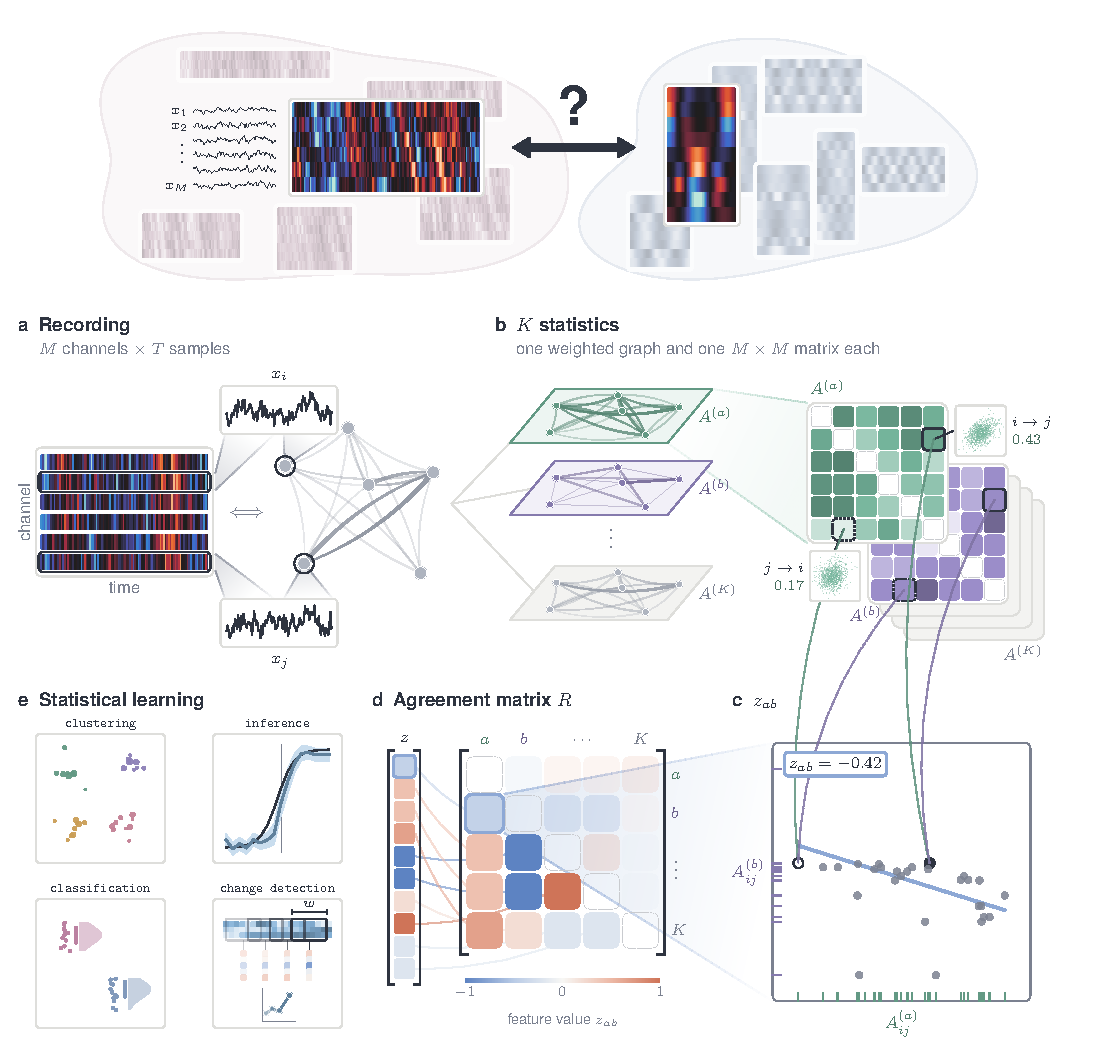
\includegraphics[width=\linewidth]{method-schematic-helvetica}	% 2026-11-18 schematic (commit cc7970a9), Helvetica rendition
	% 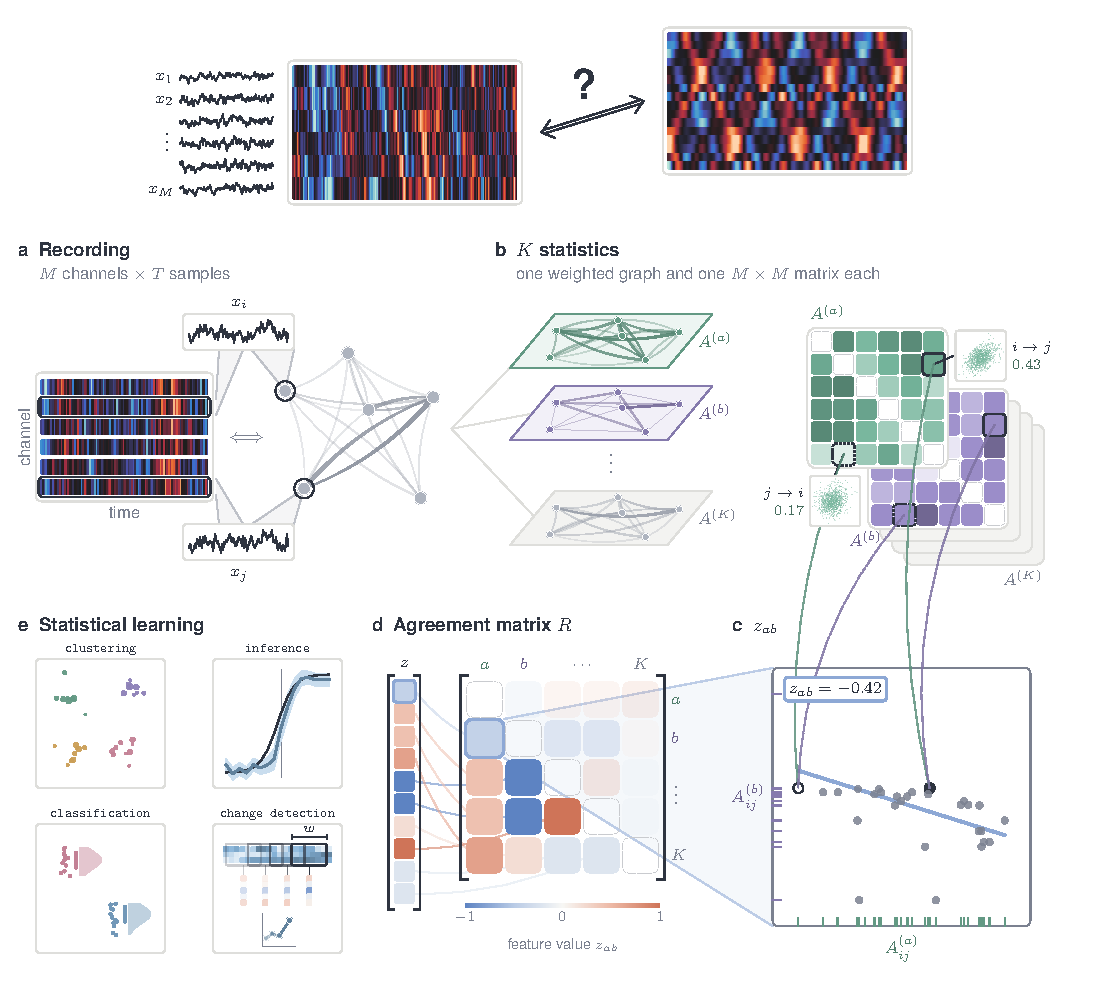
\includegraphics[width=\linewidth]{method-schematic}		% previous schematic (2026-10-30), outdated
	\caption{\textbf{The SPI--SPI representation.} \will{Placeholder caption. From an $M$-channel recording, compute every SPI over all ordered channel pairs; each SPI's edge profile is correlated with every other's to give $z_{ab}$; the vector of $z_{ab}$ is a fixed-length representation independent of $M$ and $T$.}}
	\label{fig:method}
\end{figure*}

\section{Introduction}
\textbf{Motivation: why is it important to compare multivariate time series?}
Many of the properties that distinguish complex systems are properties of how their constituents interact. Cognition, a climate teleconnection, and systemic financial risk are not attributes of a single cortical region, ocean basin, or asset's volatility \cite{bassett2017network, tsonis2004architecture, mantegna1999hierarchical}. Multivariate time series (MTS), simultaneous recordings of many interactoin univariate.

\begin{itemize}
    \item 
\end{itemize}


\section{Introduction}
\label{sec:intro}
\will{Introduction.}
Many of the properties that distinguish complex systems are properties of how their constituents interact. Cognition, a climate teleconnection, and systemic financial risk are not attributes of a single cortical region, ocean basin, or asset's volatility \cite{bassett2017network, tsonis2004architecture, mantegna1999hierarchical}. Multivariate time series (MTS), simultaneous recordings of many interacting univariate components, are the main empirical access to those interactions. Many scientific questions about such systems are therefore comparisons between multivariate time series: a young brain against an ageing one, a patient against a control, a system before and after an intervention, or two systems that may share a common organizational principle. Important information for analysis between systems may lie within individual channels, though much of it is encoded in the dependency structures \emph{between} channels -- the coupling \cite{friston2011functional, runge2019inferring}. A significant

The prevailing way to make dependence comparable is to summarise it. A pairwise statistic, such as a correlation, coherence, Granger-causal or transfer-entropy estimate, or phase-locking index, is computed for every pair of channels. The resulting matrix of coupling strengths then stands in for the recording in all downstream analysis \cite{pereda2005nonlinear,bastos2016tutorial}. When channels correspond across recordings, these matrices are compared entry by entry or through their geometry, as in connectome fingerprinting \cite{finn2015functional}, dynamic functional connectivity \cite{hutchison2013dynamic} and Riemannian classification \cite{barachant2012multiclass,dadi2019benchmarking}. When channels do not correspond, the matrix is abstracted further into mean coupling, edge-weight distributions or network topology \cite{bullmore2009complex,rubinov2010complex}, which brings its own sensitivities to network size and density \cite{vanwijk2010comparing,tantardini2019comparing}. Multilayer approaches keep several such matrices, typically one per frequency band, as the layers of one network \cite{brookes2016multilayer,buldu2018frequency}. Machine learning takes one of three routes. It infers an adjacency of interaction strengths \cite{wu2020connecting,jin2024gnn4ts}, discards cross-channel dependence by treating channels independently \cite{nie2023patchtst,han2024capacity}, or learns dependence end to end in coordinates that have no stated meaning \cite{liu2024itransformer,woo2024moirai}. Across these traditions the primitive is the same: how strongly pairs of components are coupled, under one or a few chosen notions of coupling. Each further abstraction trades information for comparability, and none can restore what the first summary removed, because any function of two identical strength matrices is identical.

Hundreds of pairwise statistics exist because dependence has many facets. It can be linear or nonlinear, instantaneous or lagged, directed or symmetric, carried by phase or by amplitude, and confined to one frequency band or spread across several. Choosing a statistic fixes, before any data are seen, the sense in which components are taken to interact; the matrix then reports how strongly they interact in that sense. Pearson correlation measures linear, zero-lag association. The phase-lag index discards zero-phase coupling by design, to suppress volume conduction \cite{nolte2004identifying,stam2007phase}. Transfer entropy depends on the history length it is given \cite{schreiber2000measuring,wibral2013measuring}. Systematic comparisons find that conclusions about network organisation, structure–function correspondence, individual identification and behavioural prediction can change substantially with the statistic \cite{smith2011network,wang2014systematic,liu2025benchmarking}. The *pyspi* library extended the highly comparative approach of univariate time-series analysis \cite{fulcher2013highly,fulcher2017hctsa} to pairwise dependence. Its more than two hundred statistics of pairwise interactions (SPIs) make the choice of statistic empirical rather than conventional \cite{cliff2023unifying}, and across tasks the best and worst statistics differ widely in performance \cite{cliff2023unifying,bryant2024extracting}. `[ALIGN: quote the published spread.]`

Choosing well does not change what is represented. A pairwise statistic compresses the relationship between two time series, a joint process with form, timing and spectral content, into one number. That map is many-to-one: relationships of very different form can share a correlation coefficient \cite{anscombe1973graphs}, and correlation summarises dependence completely only for elliptical distributions \cite{embrechts2002correlation}. Two recordings can therefore share every zero-lag correlation while their components interact differently. In one, components move together without delay; in the other, they follow one another at delays that differ from pair to pair. Every analysis built on that matrix, whether entry-wise, spectral or topological, returns the same answer for both. A change in *how* components interact is therefore not invisible to a strength representation; it is aliased. A fixed statistic registers at most a change in its value, which cannot be distinguished from a change in coupling strength, and a better statistic changes which differences are aliased, not whether some are. Such differences occur in real systems. Between wakefulness and slow-wave sleep, networks defined by zero-lag correlation are largely preserved, while the lag structure of propagated activity reorganises \cite{mitra2015propagated}. Axonal conduction delays vary systematically across the human cortex \cite{lemarechal2022atlas} and continue to shorten into adulthood \cite{vanblooijs2023developmental}. Transitions between dynamical regimes are a further case. At a synchronisation transition the coupling law stays fixed, while the observed dependence between components reorganises, for example from intermittent phase slips to sustained locking \cite{arenas2008synchronization}. Statements about such changes, that interactions became more variably delayed or changed from intermittent to locked, map onto experiments more directly than a list of edges that strengthened or weakened. Neither kind of statement identifies mechanism on its own \cite{mehler2018lure,reid2019advancing}.

The character of dependence has not been ignored, but it has been interrogated one hypothesis at a time.
- *Nonlinearity.* Surrogate-data tests ask whether a dependence exceeds what a linear Gaussian process could produce \cite{theiler1992testing,prichard1994generating,schreiber2000surrogate}. Comparisons of linear with nonlinear redundancies \cite{palus1995testing}, or of mutual information with its Gaussian counterpart, quantify nonlinear interdependence in electroencephalography \cite{breakspear2002detection} and functional magnetic resonance imaging \cite{hlinka2011functional}. Contrasts between linear and nonlinear dependence networks have characterised climate dynamics and financial crises \cite{donges2009complex,haluszczynski2017linear}.
- *Timing.* Cross-correlograms \cite{perkel1967neuronal}, lag-structure analyses \cite{mitra2014lag} and delay-resolved transfer entropy \cite{wibral2013measuring} target delays.
- *Phase versus amplitude.* Phase- and amplitude-coupling patterns have been contrasted directly \cite{engel2013intrinsic,siems2020dissociated,mostame2020phase}.
- *Redundancy versus synergy.* Information decomposition separates redundant from synergistic interaction \cite{luppi2022synergistic}.

Each of these approaches detects a change of character only if the researcher already suspects which kind of change to test. Agreement between statistics has itself been studied in two ways. Analytically, it appears as fixed relations that hold under Gaussianity and whose violation signals non-Gaussian coupling \cite{nolte2020mathematical}. Empirically, it has been measured and averaged over recordings to characterise the statistics \cite{cliff2023unifying,liu2025benchmarking}, not to describe an individual recording. A vector of per-statistic summaries can register a change of character, but only as a shift in apparent strength, and any recording-wide change in gain or signal-to-noise ratio moves all of its entries together. What such summaries discard is which channel pairs score jointly high or low across statistics. That joint organisation is where character becomes visible, and to our knowledge it has not been used to represent a recording.

We propose such a representation by inverting the role of the statistic library: rather than selecting the best statistic, we measure how statistics relate within a recording. Each statistic's values over all channel pairs of a recording form its *edge profile*. For SPIs $a$ and $b$ computed on an $M$-channel recording, $z_{ab}$ is the correlation between their edge profiles across all $M(M-1)$ ordered off-diagonal entries, so both directions of every channel pair are retained. The vector of all $z_{ab}$ is the SPI–SPI representation. A coordinate $z_{ab}$ is high when two statistics order channel pairs alike. It falls when the property that distinguishes them varies across pairs independently of shared strength. If delays vary from pair to pair, Euclidean distance and its lag-tolerant counterpart disagree about which pairs are closest. If the form of dependence varies, Pearson correlation, Spearman correlation and mutual information disagree about which pairs are most dependent. The representation therefore targets how the character of dependence is organised across a system; a change applied uniformly to every pair registers only weakly.

Because $z_{ab}$ is unchanged by positive affine rescaling of either profile, recording-wide shifts in a statistic's level or spread do not register as change. Coupling strength can still affect $z$ through the shape of the profiles. For linear Gaussian data, many coupling measures are fixed functions of coherency \cite{nolte2020mathematical}, so the spread of strength across pairs alone determines part of $z$. We therefore test readings against multivariate linear surrogates that preserve the cross-spectra, and with them that spread, together with each channel's amplitude distribution \cite{prichard1994generating,schreiber2000surrogate}, and report each reading net of its surrogate. The construction also requires heterogeneity across pairs in both profiles, and it becomes ill-conditioned when a statistic saturates. Each coordinate is indexed by two statistics with documented assumptions, which proposes a candidate interpretation. As with any multivariate readout \cite{haufe2014interpretation}, we accept that interpretation only after perturbation, surrogate and transfer tests.

Comparable second-order constructions compare neural representations \cite{kriegeskorte2008representational,kornblith2019similarity} and the layers of multiplex networks \cite{nicosia2015measuring,dedomenico2015structural}. The same across-edge correlation, applied between structural and functional connectivity, tracks brain development \cite{baum2020development}. Here the layers are alternative notions of dependence evaluated on one system.

The construction also addresses the comparability problem that motivated topological abstraction. The dimension of $z$ depends only on the number of statistics, not on the number of channels or samples. Recordings of different sizes, sensor layouts and systems therefore share one coordinate system without channel correspondence. A shared coordinate system does not by itself make positions comparable: estimates depend on recording length and channel count, and sampling must be matched to each system's timescales. We quantify these dependencies. `[ALIGN]`

We demonstrate the representation

% Methods lives in sections/methods.tex: LoG places it here, Nature after the Conclusion.
\ifnature\else
  % Methods. Input from main.tex at a style-dependent position (see \ifnature there).
% Nature (sn-jnl) asks for a single .tex at final submission: paste this back into main.tex then.
% Subsections mirror the Results; parameter values live in sections/appendix.tex.
% \will{} marks values still to be pinned.
\section{Methods}
\label{sec:methods}

\subsection{Statistics of pairwise interactions}
\label{sec:methods-spis}
A recording is a multivariate time series $X \in \mathbb{R}^{T \times M}$ of $M$ channels and $T$ samples. Each channel is $z$-scored before any statistic is computed \will{confirm per study}. A statistic of pairwise interactions (SPI) $a$ maps an ordered pair of channels $(i,j)$ to a scalar $A^{(a)}_{ij}$, giving an $M \times M$ matrix of pairwise interactions (MPI). Undirected SPIs give symmetric MPIs; directed SPIs, such as transfer entropy or Granger causality, need not. We compute SPIs with \textit{pyspi} \cite{cliff2023unifying}, using its benchmarked catalogue of $K$ statistics spanning basic, distance, causal-inference, information-theoretic, spectral and miscellaneous families \will{pin pyspi version and $K$}. The case studies use small hand-chosen subsets (\cref{sec:methods-cases}).

\subsection{The SPI--SPI representation}
\label{sec:methods-z}
For each SPI $a$, the \emph{edge profile} $\mathbf{v}_a \in \mathbb{R}^{M(M-1)}$ lists every ordered off-diagonal entry $A^{(a)}_{ij}$, $i \neq j$, in one fixed order shared by all SPIs. Both directions of every channel pair are kept, so directed SPIs retain their orientation and are compared entry by entry with undirected ones. The SPI--SPI coordinate for a pair of statistics is the Pearson correlation of their edge profiles,
\begin{equation}
	z_{ab} = \mathrm{corr}\Big(A_{ij}^{(a)}, A_{ij}^{(b)}\Big)_{i \neq j}, \qquad a,b \in \{1,\dots,K\},
	\label{eq:z-raw}
\end{equation}

or, equivalently, the cosine of their centred edge profiles,

\begin{equation}
	z_{ab} = \frac{\tilde{\mathbf{v}}_a^{\top}\tilde{\mathbf{v}}_b}{\lVert\tilde{\mathbf{v}}_a\rVert\,\lVert\tilde{\mathbf{v}}_b\rVert}, \qquad \tilde{\mathbf{v}}_a = \mathbf{v}_a - \bar{v}_a\mathbf{1},
	\label{eq:z}
\end{equation}
and the representation of the recording is the vector $\mathbf{z} = (z_{ab})_{a<b}$ of $K(K-1)/2$ coordinates. An SPI whose profile contains a non-finite entry, or has zero variance across edges, is invalid for that recording, and every coordinate involving it is missing \will{state the imputation or exclusion rule used downstream}.

Three properties follow from \cref{eq:z}. First, $z_{ab}$ is invariant to positive affine transformations of either profile, so recording-wide changes in a statistic's level or scale do not register; a sign reversal of one profile reverses the sign of $z_{ab}$. Second, $\mathbf{z}$ is invariant to any permutation applied to all profiles at once, including a relabelling of channels, so recordings need no channel correspondence and $\dim\mathbf{z}$ is independent of $M$ and $T$. Third, $\mathbf{z}$ is the upper triangle of the Gram matrix $R = B^{\top}B$ of the normalised profiles, so the full $K \times K$ matrix is positive semidefinite with rank at most $\min\{K, M(M-1)-1\}$. The construction discards each statistic's mean, scale and edge identities; what it retains is which edges the statistics rank alike. It requires heterogeneity across edges and is ill-conditioned when a statistic saturates \will{cite the saturation analysis}.

\subsection{Case studies}
\label{sec:methods-cases}
Each case study varies one property of dependence across channel pairs within a recording while holding the distribution of coupling strength fixed. Channels form three equal blocks that share one latent signal; each block is switched independently between a reference form and a modified one, and every block carries the same set of channel noise levels, so the spread of strength across edges is identical in every configuration. Each configuration is simulated in 20 independent realisations. Generator equations, parameters and SPI settings are in \cref{app:cases}.

\paragraph{Form of dependence.} Channel $i$ mixes the latent $u$ with independent noise, $w_i = (u + s_i \varepsilon_i)/\sqrt{1+s_i^2}$, and is observed through its block's map, $x_i = g(w_i)$, which is linear, monotone ($\sinh$) or non-monotone (a fold, $w^2$). Because strength enters before the map, a monotone map leaves the copula of every pair unchanged. The SPIs are Pearson correlation $r$, Spearman correlation $\rho$ and mutual information (MI), whose invariances are nested: $r$ is invariant to positive affine transformations of each variable, $\rho$ to strictly increasing ones, and MI to any invertible one.

\paragraph{Timing of dependence.} Channels are noisy readings of one smooth mother signal, $x_i(t) = m\big(t - d_i(t)\big) + \sigma_i \varepsilon_i(t)$, with delay $d_i = 0$ in an aligned block, a constant delay graded across channels in a lagged block, and a zero-mean sinusoidal delay of graded amplitude in a warped block. The SPIs are Euclidean distance (ED), its lag-tolerant counterpart (xED, the minimum Euclidean distance over integer shifts) and dynamic time warping (DTW), whose tolerances are again nested: ED tolerates no misalignment, xED a constant one, and DTW a time-varying one.

\subsection{Generative mechanisms across recording sizes}
\label{sec:methods-proof}
Nine classes from four families (independent noise, vector autoregression, Kuramoto oscillators and coupled map lattices, plus a wave equation) were simulated on a grid of channel counts and recording lengths, with ten instances per cell (\cref{app:proof}). The two variants within each family differ in one generative property at matched overall scale; for example, the two autoregressions share spectral radius and total weight and differ only in whether that weight sits on self-memory or on neighbour coupling. The full catalogue was computed on each recording. Recordings were embedded with t-SNE \will{cite openTSNE; Kobak et al.}; distances between clusters and cluster shapes in the embedding carry no meaning. Separability was checked with a five-nearest-neighbour classifier, holding out each $(M,T)$ cell in turn. For each pair of variants, one coordinate $z_{ab}$ was chosen for interpretability among those that separate the variants in every $(M,T)$ cell on a training split, and its distributions are shown on the held-out instances.

\subsection{Unsupervised inference of order parameters}
\label{sec:methods-order}
Each system is swept along one control parameter through a change of dynamical regime, and an independently defined physical order parameter $Q$ is computed from the simulated state, not from the observed channels used for $\mathbf{z}$ (systems and definitions of $Q$ in \cref{app:order}). The order coordinate $q$ is the first principal component of centred $\mathbf{z}$, fitted on development recordings only; held-out recordings are projected onto it. Every choice of preprocessing and reduction is blind to the control parameter and to $Q$, which are used only to orient the sign of $q$ for display. Agreement is reported as the Spearman correlation between $q$ and $Q$ on held-out recordings, alongside two strength baselines computed on the same recordings: mean absolute zero-lag Pearson correlation over ordered edges, and the first principal component of the per-SPI edge means.

\subsection{Software and reproducibility}
\label{sec:methods-software}
\will{pyspi version and commit; Python environment; generators, configurations and seeds in the accompanying repository; compute (NCI Gadi); data and code availability.}

\fi

\section{Results}
\label{sec:results}
\will{Results overview.}

\subsection{Case studies}
\label{sec:cases}
\will{Two minimal-pair systems in which one property of dependence is varied across channel pairs while strength is held fixed (\cref{fig:cases}).}

\subsubsection{Linear, monotone and non-monotone dependence}
\label{sec:cases-form}
Pearson correlation $r$, Spearman correlation $\rho$ and mutual information (MI) form a ladder of nested invariances: $r$ is unchanged by positive affine transformations of each variable, $\rho$ by any strictly increasing transformation, and MI by any invertible one. Each rung therefore registers a form of dependence that the rung below misreads. We built recordings in which three blocks of channels observe one latent signal, each block through its own map, with the same set of channel strengths in every block (\cref{fig:cases}, top a; \cref{sec:methods-cases}). Changing one block's map changes the form of dependence on a third of the edges and leaves the distribution of strength untouched.

When every map is linear, the three statistics rank edges alike. $z(r,\rho) = 1.00$, and $z(\rho,\mathrm{MI}) = 0.94$ (mean over 20 realisations; s.d.\ $< 0.004$). The second value sits below one because, under Gaussian dependence, MI is a convex function of correlation: the edges lie on the Gaussian curve (\cref{fig:cases}, top c, right), so the ranks agree but a Pearson-type coordinate registers the curvature. Readings are therefore relative to this reference, not to one.

Passing one block through a monotone map, $\sinh(2w)$, separates $r$ from the other two. The map leaves the copula of every pair unchanged, so $\rho$ and MI are unchanged edge by edge and $z(\rho,\mathrm{MI})$ holds at $0.94$. Pearson $r$, in contrast, is attenuated by different amounts on different kinds of edge. For jointly Gaussian inputs with correlation $c$, a monotone--linear pair has $r = \kappa c$ for a constant $\kappa < 1$, whereas a monotone--monotone pair has $r = \sinh(4c)/\sinh 4$, which compresses weak pairs far more than strong ones. The edges are reordered (\cref{fig:cases}, top c, middle), and $z(r,\rho)$ falls to $0.50 \pm 0.12$. Its larger spread across realisations reflects the heavy tails of the transformed channels, which make sample Pearson correlations unstable.

Folding one block instead, $w^2$, separates MI from the two correlations. A folded channel and a linear one are uncorrelated in population, in rank as well as in value, so $r$ and $\rho$ both assign those edges zero and continue to agree, $z(r,\rho) = 0.995$. MI still detects the dependence and assigns those edges values that grow with strength (\cref{fig:cases}, top c, right), so $z(\rho,\mathrm{MI})$ falls to $0.62 \pm 0.01$ and $z(r,\mathrm{MI})$ to $0.59$.

The two coordinates thus form a code for the form of dependence (\cref{fig:cases}, top b). A fall in $z(r,\rho)$ alone indicates monotone nonlinearity; a fall in $z(\rho,\mathrm{MI})$ alone indicates non-monotone dependence; and a recording containing both kinds of block falls in both ($z(r,\rho) = 0.87$, $z(\rho,\mathrm{MI}) = 0.62$). A per-statistic summary sees the same recordings differently. Under the monotone map the mean of $\rho$ and of MI are unchanged in population, and only the mean of $r$ drops, which cannot be told apart from weaker coupling \will{report the measured per-SPI means}. None of these contrasts is new on its own: comparing linear with nonlinear dependence measures is an established test for nonlinearity \cite{palus1995testing,hlinka2011functional}. What differs is that no comparison was chosen in advance. Both readings are coordinates of one representation, and which coordinate moves identifies the change.

\subsubsection{Instantaneous, lagged and warped dependence}
\label{sec:cases-timing}
\will{$\{\mathrm{ED}, \mathrm{XED}, \mathrm{DTW}\}$: Euclidean distance against its lag-tolerant and warping-tolerant (dynamic time warping) counterparts (\cref{fig:cases}, bottom).}

\begin{figure*}[htp]	% too tall for h or t (~0.9 page); p lets it take its own page instead of blocking later floats
	\centering
	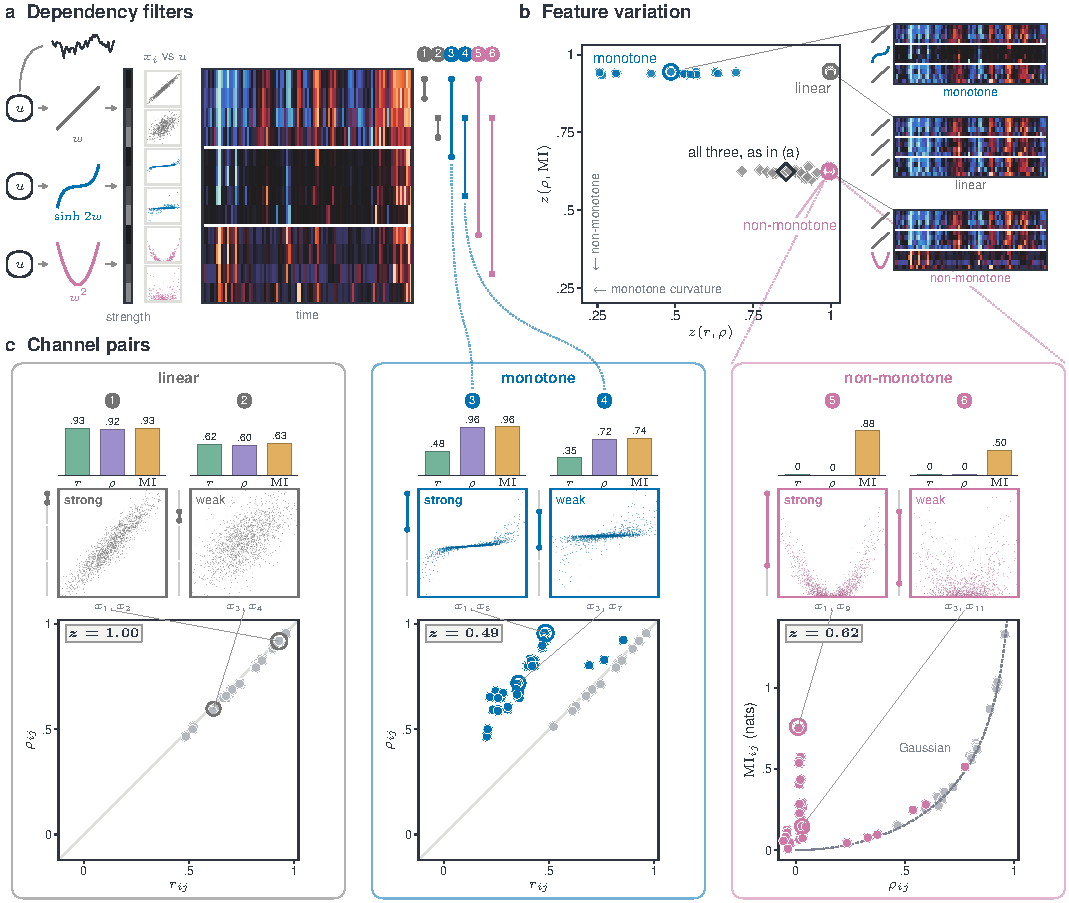
\includegraphics[width=\linewidth,height=0.45\textheight,keepaspectratio]{case-form-ladder}\par\vspace{6pt}
	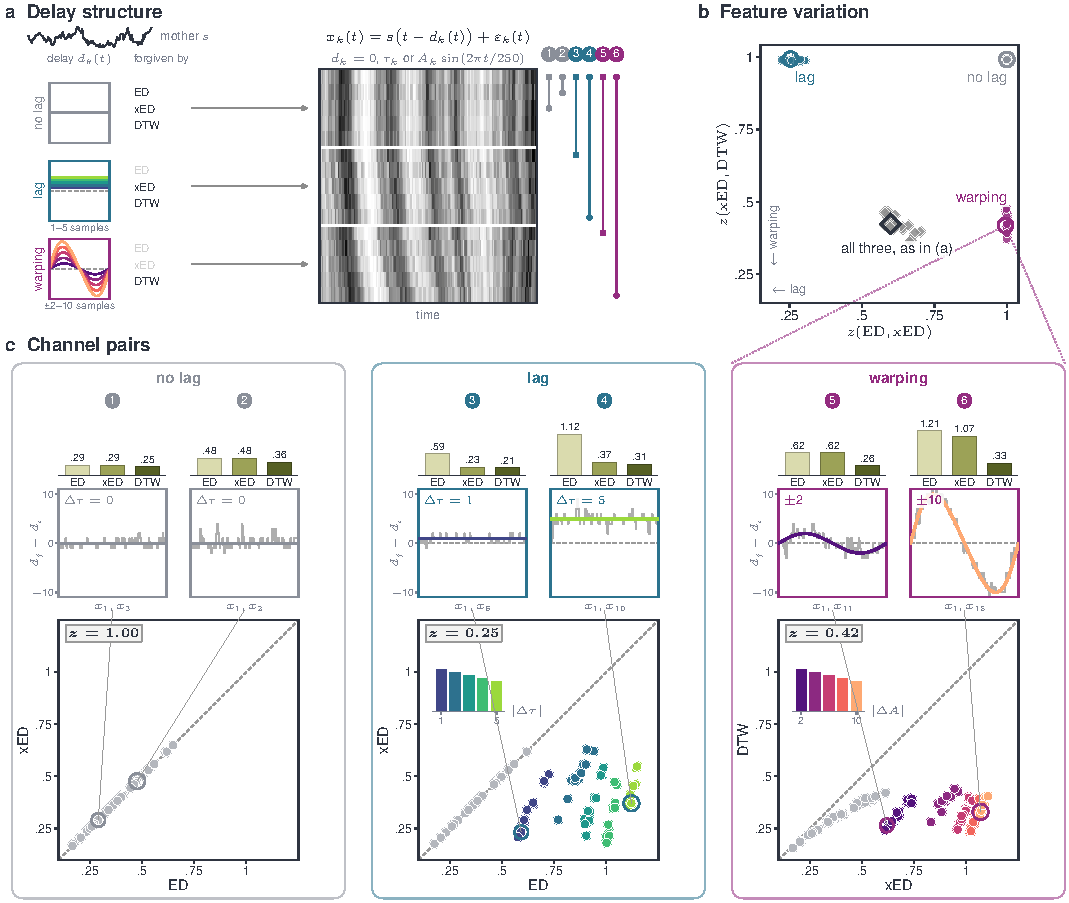
\includegraphics[width=\linewidth,height=0.45\textheight,keepaspectratio]{case-drift-blocks}
	\caption{\textbf{Pairs of statistics read the form and timing of dependence.} \will{Placeholder caption. Top: form ladder (linear, monotone, non-monotone) read by $\{r, \rho, \mathrm{MI}\}$. Bottom: delay structure (no lag, lag, warping) read by $\{\mathrm{ED}, \mathrm{XED}, \mathrm{DTW}\}$. NB both halves carry their own panels a--c; re-letter the bottom d--f at source.}}
	\label{fig:cases}
\end{figure*}

\subsection{Separating generative mechanisms across systems and recording sizes}
\label{sec:proof}
\will{Nine classes from four families (noise, VAR, Kuramoto, CML) at several $(M, T)$ form separate islands in one coordinate system; single interpretable coordinates separate the variants within each family (\cref{fig:proof}).}

\begin{figure*}[ht]
	\centering
	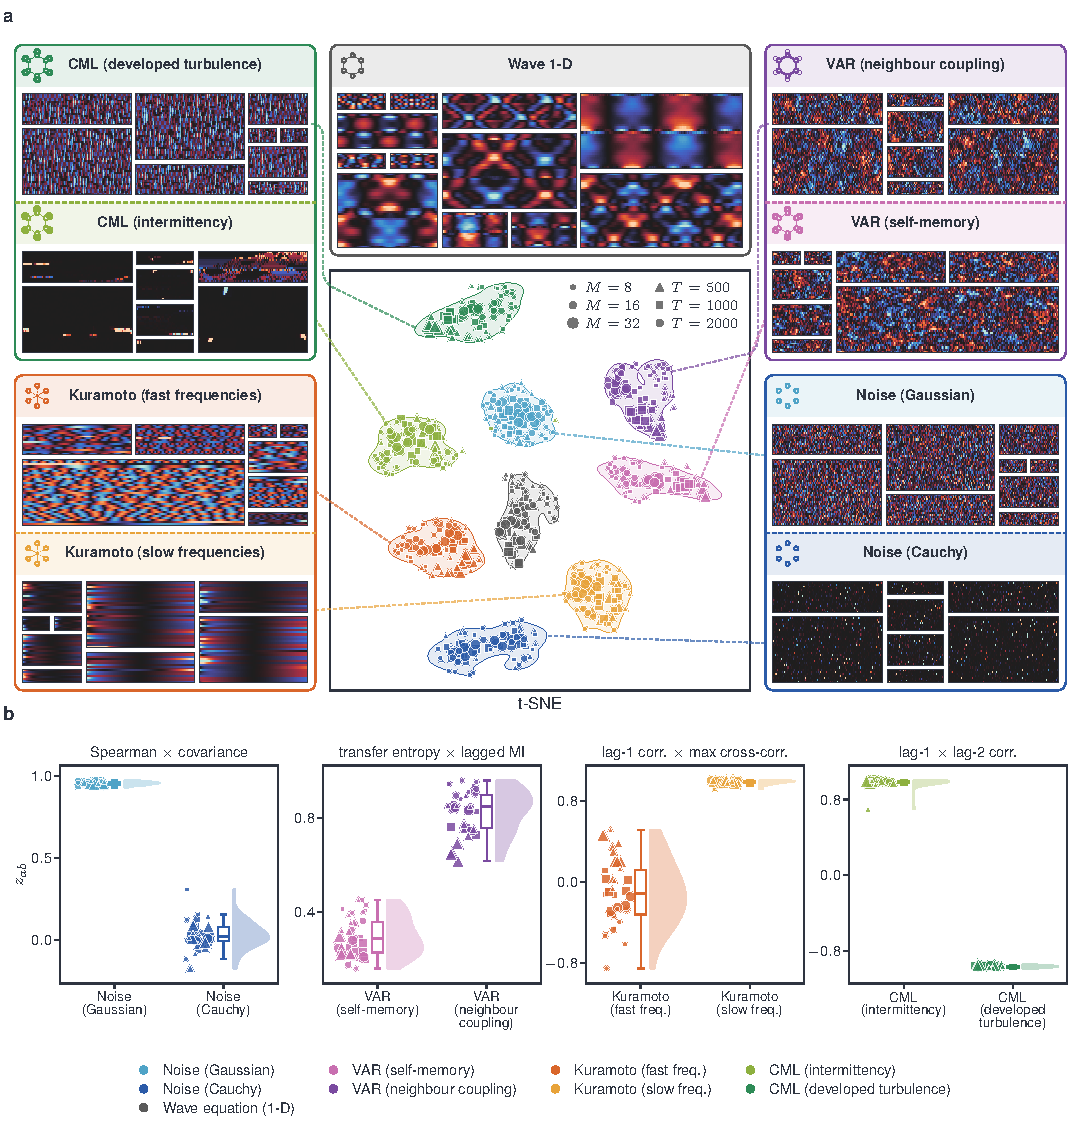
\includegraphics[width=\linewidth]{proof-of-concept}
	\caption{\textbf{One coordinate system separates generative mechanisms across recording sizes.} \will{Placeholder caption. (a) t-SNE of $z$ for nine classes; marker area encodes $M$, shape encodes $T$; carpets show example recordings of each variant, height $\propto M$ and width a time window. Two $M=8$ intermittency recordings sit with Gaussian noise: in one, all eight sites stay on the same period-3 orbit; in the other, dependence is weak and nearly uniform at $T=500$ (\cref{fig:strays}). Contour shape carries no meaning. (b) One fixed coordinate per family pair separates its variants.}}
	\label{fig:proof}
\end{figure*}

\subsection{Unsupervised inference of dynamical transitions}
\label{sec:transitions}
\will{Without labels, a coordinate of $z$ tracks the order parameter across a regime transition (\cref{fig:transitions}).}

\begin{figure*}[ht]
	\centering
	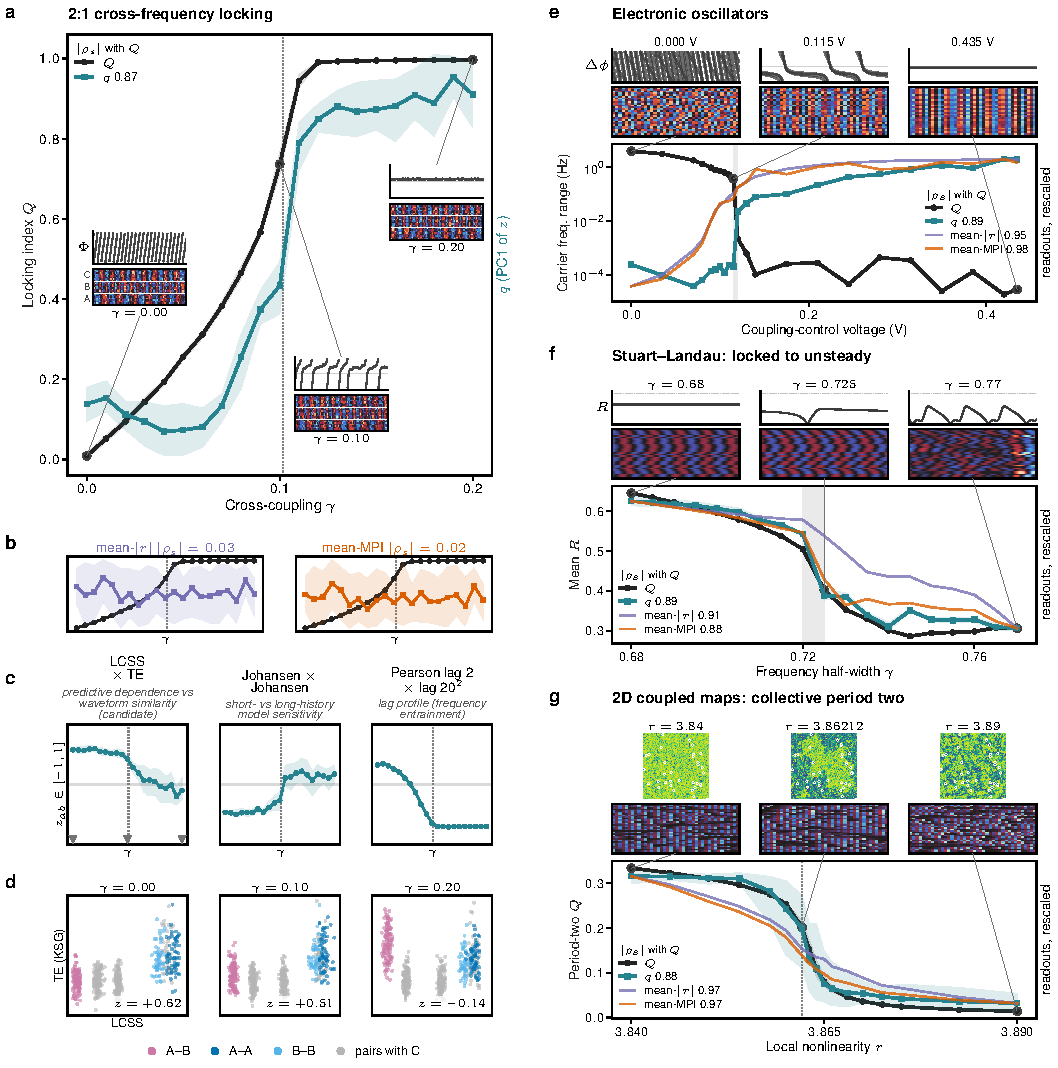
\includegraphics[width=\linewidth]{order-parameter-inference}
	\caption{\textbf{SPI--SPI coordinates infer an order parameter without supervision.} \will{Placeholder caption.}}
	\label{fig:transitions}
\end{figure*}

% Table style example (striped rows, shaded header); delete when unused.
\begin{table}
	\centering
	\caption{\textbf{Table title.} \will{Caption; table captions go above the table.}}
	\label{tab:example}
	\rowcolors{2}{white}{tablestripe} % xcolor: {odd}{even}, so data rows start striped
	\begin{tabularx}{0.8\linewidth}{@{} >{\raggedright\arraybackslash}X *{2}{>{\centering\arraybackslash}X} @{}}
		\toprule
		\rowcolor{tableheader}
		\textbf{Item} & \textbf{$n$} & \textbf{Value} \\
		\midrule
		A & 0 & 0.00 \\
		B & 0 & 0.00 \\
		C & 0 & 0.00 \\
		\bottomrule
	\end{tabularx}
\end{table}

\section{Discussion}
\label{sec:discussion}
\will{Discussion.}

\section{Conclusion}
\label{sec:conclusion}
\will{Conclusion.}

% Nature Portfolio order: Introduction, Results, Discussion, Methods.
\ifnature
  % Methods. Input from main.tex at a style-dependent position (see \ifnature there).
% Nature (sn-jnl) asks for a single .tex at final submission: paste this back into main.tex then.
% Subsections mirror the Results; parameter values live in sections/appendix.tex.
% \will{} marks values still to be pinned.
\section{Methods}
\label{sec:methods}

\subsection{Statistics of pairwise interactions}
\label{sec:methods-spis}
A recording is a multivariate time series $X \in \mathbb{R}^{T \times M}$ of $M$ channels and $T$ samples. Each channel is $z$-scored before any statistic is computed \will{confirm per study}. A statistic of pairwise interactions (SPI) $a$ maps an ordered pair of channels $(i,j)$ to a scalar $A^{(a)}_{ij}$, giving an $M \times M$ matrix of pairwise interactions (MPI). Undirected SPIs give symmetric MPIs; directed SPIs, such as transfer entropy or Granger causality, need not. We compute SPIs with \textit{pyspi} \cite{cliff2023unifying}, using its benchmarked catalogue of $K$ statistics spanning basic, distance, causal-inference, information-theoretic, spectral and miscellaneous families \will{pin pyspi version and $K$}. The case studies use small hand-chosen subsets (\cref{sec:methods-cases}).

\subsection{The SPI--SPI representation}
\label{sec:methods-z}
For each SPI $a$, the \emph{edge profile} $\mathbf{v}_a \in \mathbb{R}^{M(M-1)}$ lists every ordered off-diagonal entry $A^{(a)}_{ij}$, $i \neq j$, in one fixed order shared by all SPIs. Both directions of every channel pair are kept, so directed SPIs retain their orientation and are compared entry by entry with undirected ones. The SPI--SPI coordinate for a pair of statistics is the Pearson correlation of their edge profiles,
\begin{equation}
	z_{ab} = \mathrm{corr}\Big(A_{ij}^{(a)}, A_{ij}^{(b)}\Big)_{i \neq j}, \qquad a,b \in \{1,\dots,K\},
	\label{eq:z-raw}
\end{equation}

or, equivalently, the cosine of their centred edge profiles,

\begin{equation}
	z_{ab} = \frac{\tilde{\mathbf{v}}_a^{\top}\tilde{\mathbf{v}}_b}{\lVert\tilde{\mathbf{v}}_a\rVert\,\lVert\tilde{\mathbf{v}}_b\rVert}, \qquad \tilde{\mathbf{v}}_a = \mathbf{v}_a - \bar{v}_a\mathbf{1},
	\label{eq:z}
\end{equation}
and the representation of the recording is the vector $\mathbf{z} = (z_{ab})_{a<b}$ of $K(K-1)/2$ coordinates. An SPI whose profile contains a non-finite entry, or has zero variance across edges, is invalid for that recording, and every coordinate involving it is missing \will{state the imputation or exclusion rule used downstream}.

Three properties follow from \cref{eq:z}. First, $z_{ab}$ is invariant to positive affine transformations of either profile, so recording-wide changes in a statistic's level or scale do not register; a sign reversal of one profile reverses the sign of $z_{ab}$. Second, $\mathbf{z}$ is invariant to any permutation applied to all profiles at once, including a relabelling of channels, so recordings need no channel correspondence and $\dim\mathbf{z}$ is independent of $M$ and $T$. Third, $\mathbf{z}$ is the upper triangle of the Gram matrix $R = B^{\top}B$ of the normalised profiles, so the full $K \times K$ matrix is positive semidefinite with rank at most $\min\{K, M(M-1)-1\}$. The construction discards each statistic's mean, scale and edge identities; what it retains is which edges the statistics rank alike. It requires heterogeneity across edges and is ill-conditioned when a statistic saturates \will{cite the saturation analysis}.

\subsection{Case studies}
\label{sec:methods-cases}
Each case study varies one property of dependence across channel pairs within a recording while holding the distribution of coupling strength fixed. Channels form three equal blocks that share one latent signal; each block is switched independently between a reference form and a modified one, and every block carries the same set of channel noise levels, so the spread of strength across edges is identical in every configuration. Each configuration is simulated in 20 independent realisations. Generator equations, parameters and SPI settings are in \cref{app:cases}.

\paragraph{Form of dependence.} Channel $i$ mixes the latent $u$ with independent noise, $w_i = (u + s_i \varepsilon_i)/\sqrt{1+s_i^2}$, and is observed through its block's map, $x_i = g(w_i)$, which is linear, monotone ($\sinh$) or non-monotone (a fold, $w^2$). Because strength enters before the map, a monotone map leaves the copula of every pair unchanged. The SPIs are Pearson correlation $r$, Spearman correlation $\rho$ and mutual information (MI), whose invariances are nested: $r$ is invariant to positive affine transformations of each variable, $\rho$ to strictly increasing ones, and MI to any invertible one.

\paragraph{Timing of dependence.} Channels are noisy readings of one smooth mother signal, $x_i(t) = m\big(t - d_i(t)\big) + \sigma_i \varepsilon_i(t)$, with delay $d_i = 0$ in an aligned block, a constant delay graded across channels in a lagged block, and a zero-mean sinusoidal delay of graded amplitude in a warped block. The SPIs are Euclidean distance (ED), its lag-tolerant counterpart (xED, the minimum Euclidean distance over integer shifts) and dynamic time warping (DTW), whose tolerances are again nested: ED tolerates no misalignment, xED a constant one, and DTW a time-varying one.

\subsection{Generative mechanisms across recording sizes}
\label{sec:methods-proof}
Nine classes from four families (independent noise, vector autoregression, Kuramoto oscillators and coupled map lattices, plus a wave equation) were simulated on a grid of channel counts and recording lengths, with ten instances per cell (\cref{app:proof}). The two variants within each family differ in one generative property at matched overall scale; for example, the two autoregressions share spectral radius and total weight and differ only in whether that weight sits on self-memory or on neighbour coupling. The full catalogue was computed on each recording. Recordings were embedded with t-SNE \will{cite openTSNE; Kobak et al.}; distances between clusters and cluster shapes in the embedding carry no meaning. Separability was checked with a five-nearest-neighbour classifier, holding out each $(M,T)$ cell in turn. For each pair of variants, one coordinate $z_{ab}$ was chosen for interpretability among those that separate the variants in every $(M,T)$ cell on a training split, and its distributions are shown on the held-out instances.

\subsection{Unsupervised inference of order parameters}
\label{sec:methods-order}
Each system is swept along one control parameter through a change of dynamical regime, and an independently defined physical order parameter $Q$ is computed from the simulated state, not from the observed channels used for $\mathbf{z}$ (systems and definitions of $Q$ in \cref{app:order}). The order coordinate $q$ is the first principal component of centred $\mathbf{z}$, fitted on development recordings only; held-out recordings are projected onto it. Every choice of preprocessing and reduction is blind to the control parameter and to $Q$, which are used only to orient the sign of $q$ for display. Agreement is reported as the Spearman correlation between $q$ and $Q$ on held-out recordings, alongside two strength baselines computed on the same recordings: mean absolute zero-lag Pearson correlation over ordered edges, and the first principal component of the per-SPI edge means.

\subsection{Software and reproducibility}
\label{sec:methods-software}
\will{pyspi version and commit; Python environment; generators, configurations and seeds in the accompanying repository; compute (NCI Gadi); data and code availability.}

\fi

% ---------------------------------------------------------------------------
% BACK MATTER. LoG: remove Author Contributions and Acknowledgements for the
% [review] version; neither counts towards the page limit.
% Nature Portfolio additionally requires data/code availability and competing interests.
% ---------------------------------------------------------------------------
\ifnature
  \backmatter
  \backhead{Data availability}
  \will{Data availability statement.}

  \backhead{Code availability}
  \will{Code availability statement.}
\fi

\backhead{Author Contributions}
\will{Contributions, e.g., using CRediT (https://credit.niso.org/).}

\backhead{Acknowledgements}
\will{Acknowledgements and funding.}

\ifnature
  \backhead{Competing interests}
  The authors declare no competing interests.
\fi

% Bibliography: sn-jnl sets \bibliographystyle{sn-nature} itself (a second call breaks BibTeX).
\ifnature\else
  \bibliographystyle{unsrtnat}
\fi
\bibliography{refs}

% Appendices go after the bibliography. LoG: submitted with the main paper, the main text must be
% self-contained. Nature Portfolio: move this material to Supplementary Information / Extended Data.
\appendix
% Appendix: system parameters and settings referenced from the Methods.
% LoG: submitted after the bibliography. Nature Portfolio: becomes Supplementary Information.
\section{Case-study generators}
\label{app:cases}

\paragraph{Form of dependence.} $M=12$ channels in three blocks of four, $T=2000$. The latent $u$ is a standardised AR(1) process with coefficient $0.8$. Within every block the noise levels $s_i$ are log-spaced on $[0.2, 1]$, so the loading $1/\sqrt{1+s_i^2}$ sets each channel's strength. Maps: linear $g(w)=w$; monotone $g(w)=\sinh(2w)$, odd, so its pairs with folded channels have $r=\rho=0$ in population; fold $g(w)=w^2$. Configurations: all blocks linear; one monotone block; one folded block; one monotone and one folded block. Channels are $z$-scored after the map. SPIs: empirical covariance of the standardised channels (equal to Pearson $r$), Spearman $\rho$, and MI by the Kraskov--St\"ogbauer--Grassberger estimator \will{cite; confirm $k$}. Seed base 20261028.

\paragraph{Timing of dependence.} $M=15$ channels in three blocks of five, $T=1000$. The mother $m$ is an Ornstein--Uhlenbeck process with lag-one autocorrelation $0.9$ on a grid eight times finer than the samples, read by linear interpolation so that fractional delays do not smooth it. Lagged block: constant delays $\{1,2,3,4,5\}$ samples. Warped block: $d_i(t) = A_i \sin(2\pi t/250)$ with $A_i \in \{2,4,6,8,10\}$ samples. Observation noise $\sigma_i$ is log-spaced on $[0.1, 0.4]$ and assigned in the fixed order $(1,4,2,0,3)$ within each block, so noise does not follow lag or warp. Random draws do not depend on the block layout, so a channel whose block kind is unchanged is identical across configurations. SPIs: normalised Euclidean distance; cross-pairwise Euclidean distance, minimised over shifts up to 250 samples; unconstrained, normalised DTW. Seed base 20261029.

\section{Generative classes}
\label{app:proof}
$M \in \{8,16,32\}$, $T \in \{500,1000,2000\}$, ten instances per cell; full benchmarked catalogue \will{$K$}. VAR weights are literal: $\phi$ on self, the stated coupling on each of the two ring neighbours, so both VAR variants have total weight $0.9$.

\begin{table}[ht]
	\centering
	\caption{\textbf{Generative classes.} \will{Add generator equations; check against the proof configuration.}}
	\label{tab:classes}
	\small
	\rowcolors{2}{white}{tablestripe}
	\begin{tabularx}{\linewidth}{@{} l l >{\raggedright\arraybackslash}X @{}}
		\toprule
		\rowcolor{tableheader}
		\textbf{Family} & \textbf{Variant} & \textbf{Parameters} \\
		\midrule
		Noise & Gaussian & independent channels \\
		Noise & Cauchy & independent channels \\
		VAR & self-memory & ring, $\phi = 0.7$, neighbour coupling $0.1$ each side \\
		VAR & neighbour coupling & ring, $\phi = 0.2$, neighbour coupling $0.35$ each side \\
		Kuramoto & fast frequencies & all-to-all, $K=-4$, $\bar{\omega} = 3$, $\mathrm{sd}(\omega) = \sqrt{3}$, $\mathrm{d}t = 0.00625$ \\
		Kuramoto & slow frequencies & as above, $\bar{\omega} = 0.025$, $\mathrm{sd}(\omega) = 0.0144$ \\
		CML & intermittency & quadratic map, $\alpha = 1.7522$, $\varepsilon = 0.00115$ \\
		CML & developed turbulence & quadratic map, $\alpha = 2$, $\varepsilon = 0.3$ \\
		Wave equation & 1-D & periodic lattice, $c = 10$, five initial modes (decay $1.5$), noise sd $0.01$ \\
		\bottomrule
	\end{tabularx}
\end{table}

\paragraph{Embedding and coordinates.} t-SNE by openTSNE 1.0.4: perplexity 30, Student-$t$ kernel with five degrees of freedom, PCA initialisation, Euclidean metric, early exaggeration 12 for 250 iterations, 1250 iterations, seed 260924 \will{state the input: missing-value handling, scaling}. Separability: five-nearest-neighbour classification on the leading 50 principal components, each $(M,T)$ cell held out in turn. Raincloud coordinates: chosen among those with training AUC $\geq 0.995$ in every $(M,T)$ cell on instances 0--5; distributions show instances 6--9.

\paragraph{Intermittency recordings near noise.} Two of the 90 intermittency recordings embed with Gaussian noise (\cref{fig:proof}a); they are the only two errors of the nearest-neighbour check. Both are 8-site windows of a 100-site lattice that, as a whole, alternates between laminar and turbulent domains as intermittency should, and each window caught one extreme of the regime (\cref{fig:strays}). In one ($T=1000$), all eight sites stay on the same period-3 laminar orbit throughout, so every channel carries the same signal. Dependence is maximal, but every pair of channels is alike, and $z$, a correlation across pairs, has nothing to read. 56 of the 225 statistics do not vary across pairs, leaving 46\% of $z$ undefined; on the coordinates that remain, its ten nearest neighbours are all Gaussian noise, so the filled-in values do not place it there. Windows that are 97--99\% laminar approach the same boundary; the 99\% window, in which one site bursts 5\% of the time, stays in its island. In the other ($T=500$), the window sits on a turbulent domain that persists for the whole record. Its dependence is weak and nearly uniform across pairs, and at this size it does not rise above estimation noise: an equally weak window at $T=2000$ stays in its island, as do developed-turbulence recordings with weaker dependence at larger $M$. The two recordings lie at opposite extremes of dependence strength yet land together, so their position reflects the absence of a contrast between pairs, not the strength of dependence. $z$ alone cannot separate such recordings from noise; their dependence strengths can.

\begin{figure}[ht]
	\centering
	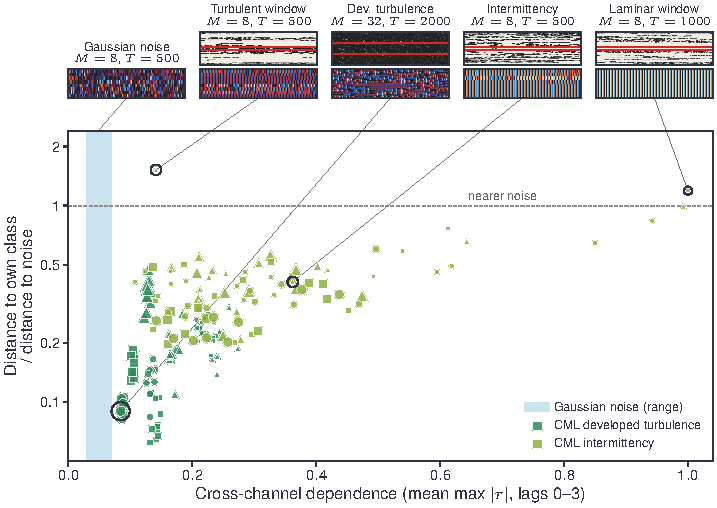
\includegraphics[width=0.7\linewidth]{proof-strays}
	\caption{\textbf{Two intermittency recordings embed with noise for opposite reasons.} Every intermittency and developed-turbulence recording of \cref{fig:proof}, by cross-channel dependence (mean over ordered channel pairs of the largest $|r|$ at lags 0--3) against its distance to its own class median divided by its distance to the Gaussian-noise median, on the leading 50 principal components; above the dashed line a recording is nearer noise. Marker area encodes $M$ and shape encodes $T$, as in \cref{fig:proof}; the shaded band spans Gaussian noise. Insets, for the circled recordings: the full 100-site lattice over the whole record (black: turbulent, $|x_t - x_{t-3}| \geq 0.05$), observed sites boxed in red, above the first 120 steps of the observed window; the Gaussian-noise inset shows one recording.}
	\label{fig:strays}
\end{figure}

\section{Order-parameter systems}
\label{app:order}
\will{One paragraph per system: model, control parameter and sweep, observation (which variables, $M$, $T$), definition of $Q$, development/held-out split. Systems: cross-frequency 2:1 locking ($M=N=24$); electronic-oscillator hardware recordings; Stuart--Landau oscillators ($M=N=32$, $T=1000$, $K=0.8$, $\gamma \in [0.68, 0.77]$); two-dimensional coupled map lattice ($L=256$, $g=0.2$, $M=32$ dispersed sites, $T=1000$).}


\end{document}
